  % Andy: For examples with posets, see: http://www.plu.edu/~edgartj/posetMobius.pdf
% Sammy, for help with the intro, use: http://www.math.miami.edu/~wachs/papers/toolnotes.pdf
% For Latex info, use http://tobi.oetiker.ch/lshort/lshort.pdf


%Wm: I think I've fixed the theorem numbering. I've also removed "from Bóna" from each theorem, definition, and proposition because Dr. Lewis said we should just state once that all of our theorems came from Bóna. I'm not sure where to say this, though. % I'll state it as a note in the abstract, but change it if you don't like it, I just did it quickly.
%Wm: I think I've fixed all the simple errors that Dr. Lewis pointed out. We still need to edit the proofs and add more explanation of why our results are significant.


\documentclass{article} %I changed this to "article" because I thought it looked better that way, but if anyone objects, feel free to change it back.% %This seems like a more formal assignment to me, so I like "report" for it, but it doesn't matter to me. I like to see things in report style first though, so change it at your discretion%Andy: I changed it back to article so our sections number correctly.
\usepackage{amsmath}
\usepackage{amsthm}
\usepackage{graphicx}
\usepackage{pslatex}
\usepackage[top=1.5in,bottom=1.5in]{geometry}
\usepackage{setspace}
\usepackage{amssymb}

\theoremstyle{definition}
\newtheorem{definition}{Definition}[section]

\theoremstyle{plain}
\newtheorem{thm}{Theorem}[section]
\newtheorem{prop}[thm]{Proposition}

\begin{document}

\begin{titlepage}
\title{\huge An Introduction to Posets} 
\author{Sammy Shaker, William Thomas, and Andrew Ylitalo}
\date{$\mathrm{22^{nd}}$ December, 2012}
\maketitle
\end{titlepage}

\begin{titlepage}

\begin{abstract}
In this paper we discuss various aspects of partially ordered sets, known as posets. In particular, we work with finite posets, that is, posets with a finite number of elements. As many combinatorial objects can be described using posets, the properties of posets we prove will allow us to achieve significant combinatorial results. We define posets and introduce some concepts and terminology fundamental to their study. We focus our attention on the zeta and M\"{o}bius functions of a poset and use them to prove the M\"{o}bius Inversion Formula, with which we derive the Principle of Inclusion-Exclusion. We also discuss lattices, a special type of poset with possessing a unique simplicity that makes them a significant area of poset theory as well. Our discussion uses many theorems and propositions found in Mikl\'{o}s B\'{o}na's \textit{A Walk Through Combinatorics}. 
\end{abstract}
\end{titlepage}

%Andy: Note that our running example is application of a concept or theorem to B_3, i.e., the poset of subsets of [3]. Having a consistent example connecting the various concepts will help the reader with understanding this subject.%
\section{Introduction}
%Smy: I'm adding more examples of posets to this introduction, as Dr. Lewis asked us to. I'm thinking of Airplane tickets and the numbers 1 through n for now, correct me if you want anything else added.
%ANDY: IDEA: I checked wikipedia and it suggested family geneology as a poset, with one element covering another if the person it represents is the other's parent. I think that might be more meaningful than the airplane ticket analogy since I believe posets are actually used in geneology.
%Andy: I think what's more important is conveying the importance of posets rather than simply conveying what they are.

The beauty of the partially ordered set, or \textit{poset}, lies in its simplicity. As its name suggests, a poset is a set of objects possessing only partial order. By this we mean that in a poset, some---though perhaps not all---pairs of elements are directly comparable. By allowing the possibility of elements that are not directly comparable, posets expand the idea of totally ordered sets---sets like that of the real numbers in which each element can be determined to be less than, equal to, or greater than any other. On the other hand, the definition of a poset is narrower than the definition of a set since a poset must have some system of order. This system of order allows for the development of mathematics surrounding these general structures. It is this mathematics that we explore in this paper, focusing our attention specifically on finite posets. The defining system of order for a poset $P$, its binary relation, denoted by $\leq$, allows the derivation of an entire field of mathematics by having all its elements follow three simple properties:
\begin{enumerate}
\item{For all $x \in P$, $x \leq x$. (Reflexivity)}
\item{If $x \leq y$ and $y \leq x$, then $x=y$. (Antisymmetry)}
\item{If $x \leq y$ and $y \leq z$, then $x \leq z$. (Transitivity)}
\end{enumerate}
The set of all subsets of $[n]$, which we call the Boolean algebra of degree $n$ and denote by $B_n$, is a classic example of a poset with the following definition for its binary relation $\leq$: if $S$ and $T$ are two different subsets of $B_{n}$, then $S \leq T$ if $S \subseteq T$. We now demonstrate that this is a suitable binary operation to make $B_{n}$ a poset by checking its compliance with the three fundamental poset criteria:
\begin{enumerate}
\item{For any subset $Q \in B_{n}$, $Q \subseteq Q$ since $Q=Q$. Thus, the binary relation $\leq$ for $B_n$ satisfies reflexivity.}
\item{Consider two elements of $B_n$, $M$ and $N$, such that $M \leq N$ and $N \leq M$. By our definition of the binary relation $\leq$, it follows that $M \subseteq N$ and $N \subseteq M$. By set theory,
%I don't believe it necessary to prove this fundamental property of set theory in a paper on posets, but if you feel we should explain this step in our logic more, feel free to add to it.
it must be true that $M=N$. Thus, $M \leq N$ and $N \leq M$ implies $M=N$ for all elements of $B_{n}$, so $\leq$ satisfies antisymmetry.}
\item{Finally, let us consider three elements $X, Y, Z \in B_n$ such that $X \leq Y$ and $Y \leq Z$. %Is this an acceptable revision of what you originally wrote? (William)%  
By the definition of the binary relation $\leq$, it follows that $X \subseteq Y$, so $Y$ contains all elements of $X$. By the same token, $Y \leq Z$ implies that $Z$ contains all elements of $Y$. Since $Y$ contains all elements of $X$, the fact that $Z$ contains all elements of $Y$ requires that $Z$ also contain all elements of $X$, so $X\subseteq Z$. By definition, $X\leq Z$. Thus, $X \leq Y$ and $Y \leq Z$ imply that $X\leq Z$, and $\leq$ satisfies transitivity.}
\end{enumerate}
Therefore, $B_n$, together with binary relation $\leq$ such that $S \leq T$ if $S \subseteq T$, is a poset. We find that $B_n$ satisfies our intuitive definition of a poset as well, that is, a set with partial order, which we will demonstrate in the case of $B_3$ (subsets of $[3]$). Its elements are:
\[
\{\}, \, \, \{1\}, \, \, \{2\}, \, \, \{3\}, \, \, \{1,2\}, \, \, \{2,3\}, \, \, \{1,3\}, \, \, \{1,2,3\}.
\] 
From the definition of our binary relation $\leq$, we determine that $\{1\} \leq \{1,2\}$, $\{1\} \leq \{1,3\}$, and all the elements are less than or equal to $\{1,2,3\}$. The element $\{1\}$, however, is neither less than or equal to nor greater than or equal to the element $\{2,3\}$: the two are incomparable elements. If we continued to determine these relationships between each pair of elements in $B_3$, we would continue to find both comparable and incomparable elements. In this way, $B_{3}$ is ``partially ordered". \\

This is only one example of a partially ordered set, and there are many others. Consider the set $[n]$ itself, along with the binary operation $x \leq y$ if the absolute value of $x$ is smaller than that of $y$. We thus have another partially ordered set with an even more natural binary operation than that of $B_{n}$. 

This method of demonstrating the partial order of a poset with the binary relation $\leq$ does not reveal much about the overall structure of a poset, and it is tedious to try to make sense out of a list of comparable and incomparable pairs of elements in a poset. Instead, it is common practice to display a poset graphically through what is called a \textbf{Hasse Diagram}. In the Hasse Diagram for a poset $P$, each element of $P$ is represented by a dot. If an element $y$ of $P$  \textbf{covers} an element $x$ of $P$, meaning that $y > x$ and there exists no $z \in P$ such that $x < z < y$, then we draw a connecting line segment between the dots of $x$ and $y$ such that the dot of $x$ is below the dot of $y$. Otherwise, there is no restriction on the location of the dots. We display the Hasse Diagram for $B_3$ below:

\begin{figure}[h!]
    \centering
        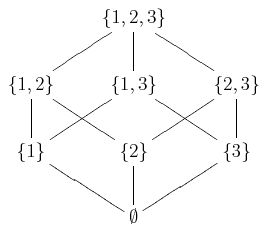
\includegraphics[scale=.75]{HasseDiagramB_3.png}
    \caption{The Hasse Diagram of $B_3$.}
\end{figure}

We note in the Hasse Diagram that although not all elements are comparable, as there exists no ordering relationship between the elements $[1]$ and $[2]$. Others, however, are comparable to all other elements; for example, it is clear that $\{1,2,3\}$ is greater than or equal to all elements in $B_3$ and that $\emptyset$ is less than or equal to all elements in $B_3$. These elements are the maximum and minimum of $B_3$, respectively. Formally, we define the \textbf{maximum} element of a poset $P$ as the element $x$ of $P$ such that $x \geq y$ for all $y \in P$. Similarly, we define that \textbf{minimum} element of a poset $P$ as the element $x$ of $P$ such that $x \leq y$ for all $y \in P$. If they exist, we denote the maximum element of a poset as $\hat{1}$ and the minimum element of a poset as $\hat{0}$, so $\{1,2,3\}=\hat{1}$ and $\emptyset=\hat{0}$ in the case of $B_3$. More generally, we define a \textbf{maximal} element of a poset $P$ as any element $x$ such that there exists no $z \in P$ for which $x < z$, and we define a \textbf{minimal} element of a poset $P$ as any element $x$ such that there exists no $z \in P$ for which $x > z$. Note that in addition to being the maximum and minimum elements of $B_3$, $\{1,2,3\}$ and $\emptyset$ are a maximal element and a minimal element, respectively.

Hasse Diagrams also reveal another characteristic of posets: although the elements of a poset are only partially ordered, there exist subsets whose elements are totally ordered. We define a \textbf{chain} to be such a collection of elements where any two elements are comparable. We also define the length of a chain $C$ as one less than the number of elements it contains, that is, $|C|-1$. One chain in $B_3$ is the set $\emptyset \leq \{1\} \leq \{1,2\} \leq \{1,2,3\}$, with length 3. A poset $P$ also has a length: the length of its longest chain. We define any chain the same length as $P$, that is, any chain such that no other chain of $P$ is longer than it, as a \textbf{maximum chain}. $B_3$, for example, has maximum chain $\emptyset \leq \{2\} \leq \{2,3\} \leq \{1,2,3\}$. Its length, and thus the length of $B_3$, is 3.\

On the other hand, there also exist subsets of a poset such that \textit{no} two elements are comparable, which we call an \textbf{antichain}. In the case of $B_3$, $\{3\}$ and $\{1,2\}$ constitute an antichain as neither of these subsets contains the other. As with chains, an antichain of a poset $P$ is a \textbf{maximum antichain} if there exists no larger antichain of $P$. \\

Chains and antichains are linked because the size of any maximum antichain of a poset $P$ is equal to the size of any smallest chain cover. A \textbf{chain cover} is any collection of disjoint chains (chains that do not share any common elements) of a poset $P$ such that their union is the poset itself, and its size is the number of chains in the chain cover. We note that one chain cover of $B_{3}$ is $\{\{1,2,3\}, \{1,2\}, \{2\}\} \cup \{ \{2,3\}, \{3\} \} \cup \{\{1,2\}, \{1\}, \emptyset \}$, with size 3. We prove the aforementioned relationship between antichains and chain covers below:

%Wm: Some of the inequalities in this proof were backwards, but I've fixed them. Does it make more sense now? Does anything still need more explanation?
\begin{thm} \textbf{Dilworth's Theorem:} In a finite poset $P$, the size of any maximum antichain is equal to the number of chains in any smallest chain cover. 
%Andy: This proof is very unclear to me. Could someone include a greater level explanation so it is more clear?
%Wm: I've revised it and included subtantially more detail than Bóna does. Is anything still unclear?
\end{thm}
\begin{proof}
%%If there are fewer chains in $B$ than elements in $A$, then the pigeon hole principle dictates that at least two elements of $A$ must be contained in one of the chains of $B$. Herein lies a contradiction since $A$ is an antichain whose elements, by definition, must not lie in any common chain. Thus, there must be no fewer chains in 
Let $A$ be a maximum antichain of $P$ and let $B$ be a smallest chain cover of $P$, that is, a chain cover with the fewest number of chains possible to include all of $P$. Denote the size of $A$ as $\alpha$ and the size of $B$ as $\beta$. There must be more chains in a smallest chain cover $B$ than elements in a maximum antichain $A$ since no two elements of $A$ can be in the same chain by the definition of an antichain. Thus $\alpha \leq \beta$.
To prove that $\beta \leq \alpha$, we will use strong mathematical induction on the number of elements of $P$, which we denote by $n$.

For $n=1$, the statement is clearly true because the single element of $P$ constitutes both the smallest chain cover and maximum antichain of $P$. Now assume that the statement is true for all $|P|<n$. We have two cases to consider:
\begin{enumerate}
\item First, assume that $P$ has a $k$-element maximum antichain $A$ with at least one non-minimal element and at least one non-maximal element. We can use $A$ to separate $P$ into two sets: $U$, the set of elements that are greater than or equal to at least one element in $A$, and $L$, the set of elements that are less than or equal to at least one element in $A$. Since $A \subseteq L,U$ and $P$ does not contain any antichains with more than $k$ elements, $A$ is a maximum antichain of $L$ and $U$. Thus by the induction hypothesis $U$ and $P$ must each be a union of $k$ chains because they are both posets with less than $n$ elements. Each of the chains in a chain cover of $U$ has one element of $A$ as its minimum, and each chain in a chain cover of $L$ has one element of $A$ as its maximum. For a given element $a$ of $A$ and chain cover of $U$ and $L$, we can form a chain from the elements of the chain in $U$ that contains $a$ and the elements of the chain in $L$ that contains $a$. Doing this for each of the $k$ elements of $A$ produces $k$ chains covering $P$. This means that the smallest chain cover of $P$ consists of at most $k$ chains. Thus we have shown that $\alpha \geq \beta$ in this case.
\item Second, assume that the maximum antichains of $P$ consist of either all maximal elements or all minimal elements. Now, let $x_1$ be a minimal element of $P$ and let $x_2$ be a maximal element of $P$ such that $x_{1} \leq x_{2}$. We can remove the elements $x_{1}$ and $x_{2}$ from $P$ to form a new poset called $P'$. This new poset has fewer than $n$ elements, and its maximum antichain cannot contain all the maximal elements or all the minimal elements of $P$ because we have removed one maximal element and one minimal element from $P$. In fact, since the maximum antichains of $P$ contained all minimal elements or all maximal elements of $P$, a maximum antichain of $P'$ must contain $k-1$ elements. Then, by the inductive hypothesis, the smallest chain cover of $P'$ has $k-1$ chains. We can then add the chain $x_{1} \leq x_{2}$ to this chain cover to produce a chain cover of $P$ with $k$ elements. This means that the smallest chain cover of $P$ consists of at most $k$ chains. Therefore, we have shown that $\alpha \geq \beta$ in this case.
\end{enumerate}

We now have that $\alpha \leq \beta$ and $\beta \leq \alpha$, and so $\beta=\alpha$. This means that the size of any maximum antichain of a finite poset $P$ is equal to the number of chains in any smallest chain cover.
\end{proof}

If we have some bijection $f: P \rightarrow [n]$, with the property that if $x < y$ in $P$ that $f(x) < f(y)$ in $[n]$, then we call this an order-perserving bijection. This is also called a \textbf{linear extension} of $P$. \\ %Wm: This could possibly be moved to Section 2.

With these basic principles of posets in mind, we can now study more interesting properties of posets. In order to work with the characteristic expressions of a poset, the zeta and M\"{o}bius functions, we first need to define an interval of a poset. An interval of a poset is defined with respect to two members of the poset; in this case, let $x, \, y \in P$. Then, the set of all $z \in P$ such that $x \leq z \leq y$ is called a \textbf{closed interval} between $x$ and $y$ of $P$ and is closed interval is represented by $[x, y]$. If all intervals of $P$ are finite, then we can call $P$ a \textbf{locally finite} poset. Note that an important property of $P$ is still undefined if it is locally finite, as $P$ can be infinite or finite. An example of a finite poset that is locally finite is $B_{3}$. An example of an infinite poset that is locally finite is the set of all positive integers with the operation $\leq$ having its classical interpretation because there is a finite number of integers between any two integers. Note that we will consider only finite (and thus also locally finite) posets in this paper. \\

%Wm: This paragraph is probably not necessary since the only place we mentioned ideals was in the statement of the Möbius Inversion Formula, but we are only working with finite posets.
%A final definition that is of importance with regards to poset theory is that of an ideal of a poset. An \textbf{ideal} of a poset $P$ is a set $I$ of $P$ for which the following property holds: if $x_{1} \in I$ and $x_{2} \leq x_{1}$, then $x_{2} \in I$. For example, the subset $D=\left[\{2, 3\}, \{2\}, \{3\}, \emptyset \right]$ of $B_{3}$ is an ideal of $B$ because every element that is $\leq$ to any element of $D$ is already contained in $D$. This example also serves another purpose; it allows for a discussion of a principal ideal. A \textbf{principal ideal} $I_{p}$ of $P$ is an ideal of $P$ that is generated using only one element. This means that $I_{p}=\{x_{1} | x_{1} \leq x_{2} \}$. The set $D$ is a principal ideal because, if we set $x_{1}=\{2,3\}$, then we can generate $D$ using the definition of an ideal. This condition on a poset is far more strict than that of being a locally finite poset; the set of all integers does not have all finite principal ideals, while the set $B_{n}$ does.


% intervals, locally finite posets, ideals, and principle ideals. Maybe also prove Theorem 16.8 from Bóna? % 

\section{Incidence Algebras and the Zeta Function} %William%

In this section we will develop the zeta function, a function useful for our investigation of posets. Though the zeta function itself is not terribly astonishing, in later sections we will use the zeta function's inverse to obtain some rather profound results.\\

First, if we let $P$ be a locally finite poset and let $Int(P)$ be the set of all intervals of $P$, then the \textbf{incidence algebra} $I(P)$ of $P$ is the set of all functions $f:Int(P) \rightarrow \bf{R}$.
The product of two functions $f \in I(P)$ and $g \in I(P)$ is defined by %Wm: Dr. Lewis's note here does not make sense to me. I(P) is the incidence algebra and Int(P) is the set of intervals of P. Andy: I think he was reading too quickly. It seems clear to me.
\begin{displaymath}
(f \cdot g)(x,y)=\sum_{x \leq z \leq y} f(x,z)g(z,y)
\end{displaymath}
Although it may not look it, this definition of multiplication functions identically to that of matrix multiplication. With any linear extension $x_1x_2 \dots x_n$ of $P$ with length $n$, we can create an $n \times n$ matrix $F$ by defining the $(i,j)$ entry as $f(x_i,x_j)$, as well as the $n \times n$ matrix $G$ by defining its $(i,j)$ entry as $G(x_i,x_j)$. The $(i,j)$ entry of the product of these matrices, $FG$, is the exact sum by which we define $(f \cdot g)(x_i,x_j)$. \\

One function in the incidence algebra of a poset is the zeta function, which we will now define.

\begin{definition}
Let $P$ be a locally finite poset. Let $\zeta \in I(P)$ be defined by $\zeta (x,y)=1$ if $x \leq y$ and $\zeta (x, y)=0$ otherwise. Then $\zeta$ is called the \textbf{zeta function} of $P$.
\end{definition}

Let $Z$ denote the zeta matrix of $P$ (i.e., the matrix whose $(i,j)$ entry is $\zeta (x_i, x_j)$). We now compute $Z$ for $B_3$.

We label the elements of $B_3$ by the linear extension $x=x_1x_2\cdots x_n$ such that $\emptyset=x_1$, $\{1\}=x_2$, $\{2\}=x_3$, $\{3\}=x_4$, $\{1,2\}=x_5$, $\{1,3\}=x_6$, $\{2,3\}=x_7$, and $\{1,2,3\}=x_8$.
%Andy: I think this might be a better way to label the elements since this is how we originally defined linear extensions.
%Wm: I dunno...where you introduced a linear extension in this way in section 4, Dr. Lewis said he didn't know what it meant. But this is the notation Bóna uses, right?
In other words, the first column and row of $Z$ will represent $\emptyset$, the second column and row will represent $\{1\}$, the third column and row will represent $\{2\}$, and so on. An entry of $Z$ will be 1 if the element of the poset represented by the row is less than or equal to the element represented by the column. Otherwise, the entry will be 0. We can use the Hasse diagram of $B_3$ to easily determine which elements are less than a given element: an element $x$ is less than an element $y$ if and only if we can travel from $x$ to $y$ along the edges of the Hasse diagram without traveling upward. For example, $\{1,2\} \leq \{1,2,3\}$, so the (4,8) entry of $Z$ will be 1. It is easy to see that

\begin{displaymath}
Z=
\begin{pmatrix}
1 & 1 & 1 & 1 & 1 & 1 & 1 & 1 \\
0 & 1 & 0 & 0 & 1 & 1 & 0 & 1 \\
0 & 0 & 1 & 0 & 1 & 0 & 1 & 1 \\
0 & 0 & 0 & 1 & 0 & 1 & 1 & 1 \\
0 & 0 & 0 & 0 & 1 & 0 & 0 & 1 \\
0 & 0 & 0 & 0 & 0 & 1 & 0 & 1 \\
0 & 0 & 0 & 0 & 0 & 0 & 1 & 1 \\
0 & 0 & 0 & 0 & 0 & 0 & 0 & 1 \\
\end{pmatrix}
\end{displaymath}

By the definition of multiplication given above, the matrix whose $(i,j)$ entry is $\zeta^2(x_i,x_j)$ is simply $Z^2$.

\begin{displaymath}
Z^2=
\begin{pmatrix}
1 & 2 & 2 & 2 & 4 & 4 & 4 & 8 \\
0 & 1 & 0 & 0 & 2 & 2 & 0 & 4 \\
0 & 0 & 1 & 0 & 2 & 0 & 2 & 4 \\
0 & 0 & 0 & 1 & 0 & 2 & 2 & 4 \\
0 & 0 & 0 & 0 & 1 & 0 & 0 & 2 \\
0 & 0 & 0 & 0 & 0 & 1 & 0 & 2 \\
0 & 0 & 0 & 0 & 0 & 0 & 1 & 2 \\
0 & 0 & 0 & 0 & 0 & 0 & 0 & 1 \\
\end{pmatrix}
\end{displaymath}

The matrix $Z^2$ allows us to determine that $\zeta^2(x_3,x_5)$ is the entry in the third row and fifth column of $Z^2$, namely 2. The values of any multiple of the zeta function, e.g. $\zeta^2$, allow us to determine properties of what we call \textit{multichains}, which we define below.

A \textbf{multichain} of a poset is defined as a multiset of elements $a_1,a_2,\dots,a_m$ satisfying $a_1 \leq a_2 \leq \cdots \leq a_m$. This is similar to the definition of a chain, but the difference between a multichain and a chain is that the elements of a multichain are not necessarily distinct. The zeta function provides us with a nice method of counting multichains.

\begin{thm} %{Bóna calls this a proposition. Can I call it a theorem?% I believe so. Dr. Lewis will correct us if we use any poor nomenclature for these statements.
Let $x \leq y$ be elements of the locally finite poset $P$. Then the number of multichains $x = x_0 \leq x_2 \leq \cdots \leq x_k = y$ (i.e., the number of multichains from $x$ to $y$ of length $k$) is equal to $\zeta^k(x,y).$
\end{thm}

\begin{proof}
We will use strong mathematical induction. If $k=1$, then the statement is true because $\zeta^1(x,y) = 1$ if $x \leq y$ and 0 otherwise, and the number of multichains of length 1 from $x$ to $y$ is also 1 if $x \leq y$ and 0 otherwise.

Assume that the statement is true for all positive integers $n<k$. Any multichain from $x$ to $y$ can be split into two multichains: $x=x_0 \leq x_1 \leq x_2 \leq \cdots \leq x_{k-1} = z$ and $z \leq y$ for some $z \in [x,y]$. By the induction hypothesis, for every $z$ the number of choices for the former is $\zeta^{k-1}(x,z)$, and the number of choices for the latter is $\zeta(z,y)$. Thus the number of multichains from $x$ to $y$ divided in this way for some fixed $z$ is $\zeta^{k-1}(x,z)\zeta(z,y)$. We can sum this over all $z$ to find that the total number of multichains from $x$ to $y$ is $\sum_{z\in [x,y]} \zeta^{k-1}(x,z) \zeta(z,y)$. By the definition of multiplication in the incidence algebra, this number is $\zeta^k(x,y)$. Therefore, by the Strong Principle of Mathematical Induction, the statement is true.
\end{proof}

For example, the (4,8) entry of $Z^2$ is 4. This means that there should be four multichains of length 2 from {3} to {1,2,3}. This is indeed true: these multichains are $\{3\}\leq\{1,3\}\leq\{1,2,3\}$, $\{3\}\leq\{2,3\}\leq\{1,2,3\}$, $\{3\}\leq\{3\}\leq\{1,2,3\}$, and $\{3\}\leq\{1,2,3\}\leq\{1,2,3\}$.

%Incidence algebras, definition of the zeta function%
%Define multichains%
%Prove Proposition 16.12%
%Example: B_3 with Hasse diagram and matrix, multichains from x_1 to x_8.%

\section{The M\"{o}bius Function} %Andy%
%Say that the matrix for the zeta function has an inverse because it's upper triangular, then define the Möbius function.%
%Prove the recursions for the Möbius function.%
%Compute the values of the Möbius function for B_3 and show the Hasse diagram with these values.%
%Example 16.19 in Bóna%

We have demonstrated that the values of the zeta function of the intervals of a poset $P$ can be organized into an $n \times n$ matrix $Z$. We now use the properties of this matrix $Z$ to determine that the zeta function has an inverse.  Let us examine the zeta matrix defined above. %Wm: I removed the sentences Dr. Lewis said were redundant. Does this transition make it sound like we're talking about B_3?%

By the definition of a linear extension, it is only possible that $x_i \leq x_j$ if $i < j$, so $i < j$ implies that $x_j \not\leq x_i$. As the row number $i$ is less than the column number $j$ for all entries below the main diagonal, entries below the main diagonal in $Z$ are all 0s, so $Z$ is upper triangular. Since $x_i \le x_j$ if $i=j$, $\zeta(x_i,x_j)=1$ when $i=j$, so all the entries along the main diagonal of Z are 1s. The determinant of an upper triangular matrix is the product of the entries along its main diagonal; therefore, $det(Z)=1$. Any matrix with a nonzero determinant has an inverse matrix, so $Z$ has inverse matrix $Z^{-1}$. As $Z$ is a matrix defined by the $\zeta$ function of $P$, there must be function that is the inverse of the $\zeta$ function associated with the matrix $Z^{-1}$. %explain further? I can't think of how. Andy: Is this better?
We call this inverse function the M\"{o}bius function of $P$, which we will signify by $\mu$.\\

Just as we can define a matrix $Z$ by the values of the zeta function, we can also define the matrix $M$ by the values of the M\"{o}bius function such that its $(i,j)$ entry is equal to $\mu(x_i,x_j)$. Since the M\"{o}bius function is the inverse of the zeta function, it follows that $M=Z^{-1}$. Since the inverse of an upper triangular matrix is upper triangular as well, we determine that $M$ is upper triangular like its inverse $Z$. Given this property of the matrix $M$, it follows that all entries below the main diagonal, that is, all entries $(i,j)$ where $i \not \leq j$, are 0. Since the $(i,j)$ entry of the matrix $M$ is equal to $\mu(x_i,x_j)$ by our definition of $M$, $\mu(x_i,x_j)=0$ if $i \not \leq j$. By the definition of the matrix $M$, these entries are also equal to $\mu(x_i,x_j)$, where $x_i \not\leq x_j$ by the definition of a linear extension. Thus, we determine that $\mu(x_i,x_j)=0$ if $x_i \not\leq x_j$. We can also determine that since $Z$ has 1s along its main diagonal and is upper triangular, $M$ also must have 1s along its main diagonal in addition to being upper triangular. Since the entries along the main diagonal of $M$ have $i=j$, it follows from the definition of $M$ that $\mu(x_i,x_i)=1$. We are now in a position to prove the following recursion regarding the remaining values of the M\"{o}bius function.

\begin{thm} Let $P$ be a locally finite poset. Let $[x,y] \in Int(P)$. Then
$$\mu(x,y)=-\sum_{x\le z<y}\mu(x,z) $$
if $x < y$.
\end{thm}
\begin{proof} Since $\zeta$ and $\mu$ are inverse functions in the incidence algebra of $P$, $(\mu\zeta)(x,y)=\delta(x,y)$, where $x$ and $y$ are elements of $P$. The definition of multiplication in the incidence algebra of $P$ also shows that
$$(\mu\zeta)(x,y)=\sum_{x\le z\le y}\mu(x,z)\zeta(z,y).$$
By substitution, we have that
$$\sum_{x\le z\le y}\mu(x,z)\zeta(z,y)=\delta(x,y).$$
Since $z \le y$ for all $z$ in the summation, $\zeta(z,y)=1$, so our equation becomes
$$\sum_{x\le z\le y}\mu(x,z)=\delta(x,y).$$
If we look specifically at the case where $x<y$, it follows that $\delta(x,y)=0$ by definition. Thus, if $x<y$,
\begin{align*}
\sum_{x\le z\le y}\mu(x,z)=&0\\
\sum_{x\le z<y}\mu(x,z)+\mu(x,y)=&0\\
\mu(x,y)=&-\sum_{x\le z<y}\mu(x,z).
\end{align*}
Therefore, if $x<y$, then $\mu(x,y)=-\sum_{x\le z<y}\mu(x,z)$ for a
%locally finite
poset $P$.
\end{proof}

Using this recursion and the facts that $\mu(x,y)=0$ if $x \not\leq y$ and $\mu(x,x)=1$, we can calculate the value of the M\"{o}bius function for any pair of elements in a poset. For example, returning to the case of $B_3$,
%
%Andy: Should we get rid of this picture and simply refer the reader to figure 1, which is identical but found a few pages earlier? Wm: I think so.
%
\begin{center}
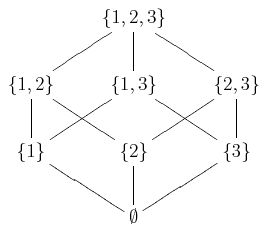
\includegraphics[scale=.75]{HasseDiagramB_3.png}
\end{center}
if we label the elements of $B_3$ such that $\emptyset=x_1$, $\{1\}=x_2$, $\{2\}=x_3$, $\{3\}=x_4$, $\{1,2\}=x_5$, $\{1,3\}=x_6$, $\{2,3\}=x_7$, and $\{1,2,3\}=x_8$, and we define the matrix $M$ representing the values of the M\"{o}bius function as we have above, we have that
\begin{displaymath}
M=
\left(\begin{array}{rCCCCCCCCl}
1&-1&-1&-1&1&1&1&-1\\
0&1&0&0&-1&-1&0&1\\
0&0&1&0&-1&0&-1&1\\
0&0&0&1&0&-1&-1&1\\
0&0&0&0&1&0&0&-1\\
0&0&0&0&0&1&0&-1\\
0&0&0&0&0&0&1&-1\\
0&0&0&0&0&0&0&1
\end{array}\right)
\end{displaymath}

Although we calculated the values of the M\"{o}bius function for $B_3$ using what we deduced above, the case of $B_n$ serves as a special case that can be described with a closed formula.
\begin{thm} Let $P=B_n$, and let $S$ and $T$ be two elements of $P$, that is, two subsets of $[n]$, such that $S \subseteq T$. Then
$\mu(S,T)=(-1)^{|T-S|}.$
\end{thm}
\begin{proof} We first define $k=|T-S|$. We then prove that $\mu(S,T)=(-1)^{k}$ for $k \ge 0$ by strong induction.\\\\
1. \textit{Base Case:} $k=0$. \\

When $k=0$, $|T-S|=0$, so $S$ and $T$ have the same elements and are thus the same set. By definition, the M\"{o}bius function of a pair of identical elements of a poset is 1, so $\mu(S,T)=1$. By our formula, $(-1)^{k}=(-1)^0=1$. Thus, our formula holds for the base case. \\\\
2. \textit{Assume that $\mu(S,T)=(-1)^{i}$ where $|T-S|=i$ whenever $0\le i\le k-1$.} \\\\
3. \textit{Prove true the $k$ case, that is, that $\mu(S,T)=(-1)^k$.}\\\\

Since $|T-S|=k$, there are $k$ elements of $T$ not in $S$. There are $\binom{k}{i}$ ways to choose $i$ of these $k$ elements and place them into $S$ to create a new subset of $[n]$. We denote any such set created in this manner as $S_{i}$, where $i$ is the number of elements added to $S$. Each of the these $S_i$ contains $|S|+i$ elements. We know from Theorem 3.1 that
$$\mu(S,T)=-\sum_{Y\in[S,T)}\mu(S,Y).$$
All $Y\in[S,T)$ are subsets of $[n]$ comprised of the elements of $S$ and up to $k-1$ of the elements in $T$ and not in $S$. This set of subsets $Y$, however, is identical to the set of subsets $S_i$ with $i\in[0,k-1]$. Since there are $\binom{k}{i}$ subsets $S_i$, substitution gives that
$$\mu(S,T)=-\sum_{i=0}^{k-1}\binom{k}{i}\mu(S,S_i).$$
By our assumption, we have $\mu(S,S_{i})=(-1)^{|S_i-S|}=(-1)^{|S|+i-|S|}=(-1)^i$. Substitution into our equation gives us that
\begin{align*}
\mu(S,T)=&-\sum_{i=0}^{k-1}\binom{k}{i}(-1)^i\\
=&(-1)^k-\left\sum_{i=0}^{k}\left\binom{k}{i}(-1)^i\right\right\\ %Wm: I rewrote this to make it easier to read.
=&(-1)^k-(1-1)^k \qquad \text{Binomial Theorem}\\
=&(-1)^k,
\end{align*}
as needed.\\\\
Therefore, by the strong principle of mathematical induction, if $P=B_n$ and $S\subseteq T\subseteq B_n$, then $\mu(S,T)=(-1)^{|T-S|}$.
\end{proof}
If we apply this formula to the first few values of the M\"{o}bius function of $B_3$, we find that the values calculated earlier by the recursion satisfy the values given by our new formula.


\section{The M\"{o}bius Inversion Formula} %Andy%
%Begin with a transitional example similar to p. 392 in Bóna.%
%Prove the Möbius Inversion Formula.%
%Use the Möbius Inversion Formula to prove the Inclusion-Exclusion formula.%
Having determined how to calculate the values of the M\"{o}bius function, we are in a position to determine uses of this function. Many of its uses stem from the following result regarding scalar functions of posets, known as the \textit{M\"{o}bius Inversion Formula}, which we prove below.
\begin{thm}
\textbf{The M\"{o}bius Inversion Formula:} Given a poset $P$,
%noting that we are only discussing finite posets
let $f$ be a function $f:P\rightarrow \mathbb{R}$ and define the function $g:P\rightarrow \mathbb{R}$ such that
$$g(y)=\sum_{x\le y}f(x).$$
Then
$$f(y)=\sum_{x\le y}g(x)\mu(x,y).$$
\end{thm}
\begin{proof} Denote the number of elements in $P$ as $n$ and create a linear extension of the elements of $P$, labeling the element assigned the integer $i$ as $x_i$. We define the row vector \textbf{f} such that
$$\textbf{f}=\begin{bmatrix}
f(x_1) & f(x_2) & \cdots & f(x_n)
\end{bmatrix},$$
and in the same way define the row vector \textbf{g}:
$$\textbf{g}=\begin{bmatrix}
g(x_1) & g(x_2) & \cdots & g(x_n)
\end{bmatrix}.$$
Since the $\zeta$ function is defined such that $\zeta(x,y)=1$ if $x\le y$ and 0 if otherwise, $\zeta(x,y)=1$ for all $x$ considered in the sum that defines $g$. Thus, we can multiply this sum by $\zeta(x,y)$ without affecting its validity, giving us that
$$g(y)=\sum_{x\le y}f(x)\zeta(x,y).$$
Since the multiplication of functions of posets is identical to the multiplication of their matrices, we rewrite the equation above in terms of the matrices of the functions, so we have that
$$\textbf{g}=\textbf{f}\cdot Z$$ 
where $Z$ is the matrix representing the values of the $\zeta$ function defined earlier. Given that $M$ -- the matrix representing the values of the M\"{o}bius function -- is the inverse of $Z$, we have the following result when we multiply on the right by $M$:
$$\textbf{g}\cdot M=\textbf{f}.$$
If we rewrite this multiplication of matrices in terms of functions, we have
$$\sum_{x\le y}g(x)\mu(x,y)=f(y).$$
Therefore, $g(y)=\sum_{x \le y}f(x)$ implies that $f(y)=\sum_{x \le y}g(x)\mu(x,y).$
\end{proof}
The M\"{o}bius Inversion Formula extends our understanding of the behavior of a pair of functions defined according to its hypothesis. By defining these functions appropriately for a poset, one can illuminate the understanding of the poset's structure with the M\"{o}bius Inversion Formula as well. In fact, the proper definition of $f$ and $g$ for the poset $B_n$ allows us to use the M\"{o}bius Inversion Formula to derive the Principle of Inclusion-Exclusion for a collection of sets $A_1,A_2,\ldots,A_n$. To do so, however, requires us to use the corollarly of the M\"{o}bius Inversion Formula, which we state below:
\begin{thm} \textbf{Corollary to the M\"{o}bius Inversion Formula:} Given a poset $P$,
%noting that we are only discussing finite posets
let $f$ be a function $f:P\rightarrow \mathbb{R}$ and define the function $g:P\rightarrow \mathbb{R}$ such that
$$g(y)=\sum_{x\ge y}f(x).$$
Then
$$f(y)=\sum_{x\ge y}g(x)\mu(y,x).$$
\end{thm}
The proof of this corollary follows a line of logic symmetric to that of Theorem 4.1. The principle difference is that we define \textit{column} vectors for the functions $f$ and $g$ as we did row vectors in the previous proof. Because of this difference, in the step where we multiply by $M$, we multiply on the left in this case rather than on the right.\\

%Is everyone okay with deleting this proof?
%Andy: yes, but I'm adding a little more to our proof sketch.
%\begin{proof} Again, denote by $n$ the number of elements in $P$, create a linear extension of the elements of $P$, and label these %elements $x=x_1x_2\ldots x_n$ such that the element assigned the integer $i$ in the linear extension is labeled $x_i$. In this proof, %however, we define the \textit{column} vector 
%$\textbf{f}=\begin{bmatrix}
%f(x_1)\\
%f(x_2)\\
%\vdots\\
%f(x_n)
%\end{bmatrix}$\\
%and in the same way define the column vector \textbf{g}:
%$\textbf{g}=\begin{bmatrix}
%g(x_1)\\
%g(x_2)\\
%\vdots\\
%g(x_n)
%\end{bmatrix}$\\
%From the definition of $g(y)$ we have that
%$$g(y)=\sum_{x\ge y}f(x).$$
%Since the $\zeta$ function is defined by $\zeta(x,y)=1$ if $x\le y$ and 0 if otherwise, the $\zeta$ function is equal to 1 for are $x$ %considered in this sum that defines $g$. Thus, we can multiply $f(x)$ by $\zeta(x,y)$ without changing the equation:
%$$g(y)=\sum_{x\ge y}\zeta(x,y)f(x).$$
%As before, we can rewrite this multiplication of functions in the incidence algebra of $P$ in matrix form:
%$$\textbf{g}=Z\textbf{f}.$$
%As $M$ is the inverse of $Z$, we get the following when multplying on the left by $M$:
%$$M\textbf{g}=\textbf{f}.$$
%If we reverse our earlier procedure, now rewriting this multiplication of matrices in function format, we have
%$$\sum_{x\ge y}\mu(y,x)g(x)=f(y).$$
%Therefore, $g(y)=\sum_{x\ge y}f(x)$ implies that $f(y)=\sum_{x\ge y}g(x)\mu(y,x).$
%\end{proof}

This result will serve as the basis of the following proof of the Principle of Inclusion-Exclusion:

%For example, given poset $B_n$, define functions $f:B_n\rightarrow \mathbb{R}$ and $g:B_n\rightarrow \mathbb{R}$ such that, if $S,T\subseteq B_n$,
%$$g(T)=\sum_{T \subseteq S}f(S).$$
%By the definition of $B_n$, we have that
%$$g(T)=\sum_{T \leq S}f(S).$$
%Now we can apply the corollary to the M\"{o}bius Inversion Formula we just proved, giving us
%$$f(T)=\sum_{T \leq S}g(S)\mu(T,S).$$
%Applying our earlier result regarding the M\"{o}bius function of subsets of $B_n$, we have that
%$$f(T)=\sum_{T \subseteq S}g(S)(-1)^{|S-T|}.$$ %This needed a g(S), right?
%This result allows us to use the M\"{o}bius function to calculate the values of the function $f$ from $g$. One very special case produces a familiar theorem:
\begin{thm} \textbf{The Principle of Inclusion-Exclusion:} Let $A_1,A_2,\ldots,A_n$ be finite sets. Then 
$$|A_1\cup A_2 \cup \cdots \cup A_n|=\sum_{j=1}^n(-1)^{j-1}\sum_{i_1,i_2,\ldots,i_j}|A_{i_1}\cap A_{i_2}\cap \cdots \cap A_{i_j}|,$$
where $(i_1, i_2,\ldots,i_j)$ ranges over all $j$-element subsets of $[n]$.
\end{thm}
\begin{proof} We begin by defining the poset $P$ as the Boolean algebra $B_n$, ordering elements $S$ and $T$ of $B_n$ such that $S\leq T$ if $S\subseteq T$. We next define the universal set $U$ such that $A_1\cup A_2 \cup \cdots \cup A_n=U$. All elements we consider will be part of this universal set. To use the results of the M\"{o}bius Inversion Formula, we must define the appropriate functions, so we define functions $f:B_n\rightarrow \mathbb{R}$ and $g:B_n\rightarrow \mathbb{R}$ as follows:
$$f(T)=\left|\bigcap_{i\in T}A_i\diagdown\bigcup_{j\in [n]\diagdown T}A_j\right|$$
and
$$g(T)=\sum_{T \le S}f(S).$$
In the case of $B_3$, $f({2,3})$ and $f({1,2,3})$ count the number of elements contained in the sets marked in the figure below:

%Wm: I shrank this figure in order to make it fit on the correct page.
\begin{figure}[h!]
    \centering
        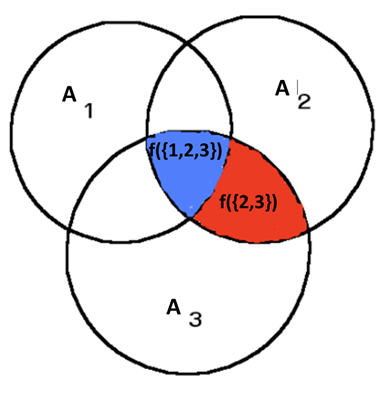
\includegraphics[scale=.75]{Inclusion-Exclusion(small).png}
    \caption{The elements counted by $f(\{1,2,3\})$ and $f(\{2,3\})$.}
\end{figure}

We call the elements counted by $f(T)$ those ``uniquely contained" by the set of all $A_i$ such that $i\in T$. That is to say that $f(T)$ counts the elements contained in all $A_i$ for $i\in T$ but \textit{not} contained in any $A_j$ for $j\in [n]\diagdown T$. By this definition of ``uniquely contained," we call the region marked by $f(\{2,3\})$ in Figure 2 the set of all elements uniquely contained by $A_2$ and $A_3$. Similarly, the region marked $f(\{1,2,3\})$ is the set of all elements uniquely contained by $A_1$, $A_2$, and $A_3$. 
%Thus, we can interpret $f(T)$ as giving the number of elements contained only by each $A_i$ such that $i\in T$ and no other sets $A_j$. In investigating the meaning of $g$, we note that, by the ordering of $B_n$, the set of all elements $S$ of $B_n$ such that $S\geq T$ is the set of all subsets of $[n]$ that include the elements of $T$. 
%We note that in this definition of $f$, $f(\emptyset)=|U-A_1\cap A_2\cap \ldots \cap A_n|$ as the only restriction on elements counted by $f(\emptyset)$ is the restriction that $x\not\in A_j \text{where }j\in[n]$ and $U$ is the universal set. This fact suggests that finding an expression for $f(\emptyset)$ will allow us to calculate the value of the intersection of all $A_i$.
The elements counted by $g$ merit no special name, however: $g(T)$ counts the number of elements in the intersection of all $A_i$ such that $i\in T$.

We prove that $g(T)=\left|\bigcap_{i\in T}A_i\right|$ in three steps: 
\begin{enumerate}
\item{We prove that $$\bigcap_{i\in T}A_i\subseteq \bigcap_{i\in S}A_i-\bigcup_{j\in [n]\diagdown S}A_j$$ for some $S\in B_n$ such that $T\subseteq S$.}
\item{We prove that 
$$\bigcap_{i\in S}A_i\diagdown\bigcup_{j\in [n]\diagdown S}A_j\subseteq \bigcap_{i\in T}A_i$$ for all $S\in B_n$ such that $T\subseteq S$.} 
\item{We prove that if $$\bigcap_{i\in S_1}A_i\diagdown\bigcup_{j\in [n]\diagdown S_1}A_j=\bigcap_{i\in S_2}A_i\diagdown\bigcup_{j\in [n]\diagdown S_2}A_j$$ for some $S_1,S_2\in B_n$, then $S_1=S_2$.}
\end{enumerate}
The combination of the first and second will prove that $\left|\bigcap_{i\in T}A_i\right|=\left|\bigcup_{T\subseteq S}\left(\bigcap_{i\in S}A_i-\bigcup_{j\in [n]\diagdown S}A_j\right)\right|$. The third will prove that summing $\left|\bigcap_{i\in S}A_i-\bigcup_{j\in [n]\diagdown S}A_j\right|$ for all $S\in B_n$ such that $T\subseteq S$ will give us precisely $\left|\bigcap_{i\in T}A_i\right|$ with no double-counted elements, that is, that $\left|\bigcap_{i\in T}A_i\right|=\sum_{T\subseteq S}\left|\bigcap_{i\in S}A_i-\bigcup_{j\in [n]\diagdown S}A_j\right|$. Given our definitions of $f$ and $g$, substitution into this equation will give us that $g(T)=\left|\bigcap_{i\in T}A_i\right|$.
\begin{enumerate}
\item{To prove that $\bigcap_{i\in T}A_i\subseteq \bigcup_{T\subseteq S}\left(\bigcap_{i\in S}A_i-\bigcup_{j\in [n]\diagdown S}A_j\right)$, we must show that for all $x\in \bigcap_{i\in T}A_i$, there exists some $S\in B_n$ for which $T\subseteq S$ such that $x\in \bigcap_{i\in S}A_i-\bigcup_{j\in [n]\diagdown S}A_j$. Given $x\in\bigcap_{i\in T}A_i$ for some $T\in B_n$, we can determine for $x$ the largest set $S\in B_n$ such that $x\in A_i$ for all $i\in S$. It follows from $x\in\bigcap_{i\in T}A_i$ that $x\in A_i$ for all $i\in T$ as well; however, $T$ is not necessarily the largest set such that $x\in A_i$ for all $i\in T$, so $T\subseteq S$. Since $x$ can only either be in a set $A_i$ or not in a set $A_i$, and since $S$ is the largest set such that $x\in A_i$ for all $i\in S$, it follows that $x\not\in A_j$ for all $j\in [n]\diagdown S$. Thus, $x\in\bigcap_{i\in S}A_i\diagdown\bigcup_{j\in [n]\diagdown S}A_j$ for any $x\in \bigcap_{i\in T}A_i$. Therefore, there exists some $S\in B_n$ such that $T\subseteq S$ for which $\bigcap_{i\in T}A_i\subseteq \bigcup_{T\subseteq S}\left(\bigcap_{i\in S}A_i\diagdown\bigcup_{j\in [n]\diagdown S}A_j\right)$ for all $T\in B_n$.}
\item{To prove the converse, that is, that $\bigcap_{i\in S}A_i\diagdown\bigcup_{j\in [n]\diagdown S}A_j\subseteq \bigcap_{i\in T}A_i$ for all $S\in B_n$ such that $T\subseteq S$, we show that if $x\in \bigcap_{i\in S}A_i\diagdown\bigcup_{j\in [n]\diagdown S}A_j$ for some $S\in B_n$ such that $T\subseteq S$, then $x\in \bigcap_{i\in T}A_i$. Given such an $x$, we can state more generally that $x\in \bigcap_{i\in S}A_i$. By the definition of an intersection, $x\in A_i$ for all $i\in S$. Since $T\subseteq S$, it follows that $x\in A_i$ for all $i\in T$ as well. Thus, $x\in \bigcap_{i\in T}A_i$. Therefore, for all $S\in B_n$ such that $T\subseteq S$, $\bigcap_{i\in S}A_i\diagdown\bigcup_{j\in [n]\diagdown S}A_j\subseteq \bigcap_{i\in T}A_i$. Since there exists some $S\in B_n$ such that $T\subseteq S$ for which $\bigcap_{i\in T}A_i\subseteq \bigcup_{T\subseteq S}\left(\bigcap_{i\in S}A_i\diagdown\bigcup_{j\in [n]\diagdown S}A_j\right)$ for all $T\in B_n$, and since two sets that are subsets of each other have the same (and same number of) elements, it follows that $\left|\bigcap_{i\in T}A_i\right|=\left|\bigcup_{T\subseteq S}\left(\bigcap_{i\in S}A_i\diagdown\bigcup_{j\in [n]\diagdown S}A_j\right)\right|$.}
\item{We prove our final result using an indirect proof in which we assume that there exist distinct $S_1,S_2\in B_n$ such that $T\subseteq S_1, S_2$ for which there is some element $x$ such that $x\in\bigcap_{i\in S_1}A_i\diagdown\bigcup_{j\in [n]\diagdown S_1}A_j$ and $x\in\bigcap_{i\in S_2}A_i\diagdown\bigcup_{j\in [n]\diagdown S_2}A_j$. Given this assumption, it must follow that there exists some integer $i^*\in [n]$ contained in either $S_1$ or $S_2$ but not contained in the other. Since our definition of $S_1$ and $S_2$ does not distinguish between the two, let $i^*\in S_1$ and $i^*\not\in S_2$; then $i^*\in [n]\diagdown S_2$. Since $x\in\bigcap_{i\in S_1}A_i\diagdown\bigcup_{j\in [n]\diagdown S_1}A_j$, we can state more generally that $x\in\bigcap_{i\in S_1}A_i$, so $x\in A_{i^*}$ since $i^*\in S_1$. On the other hand, since $x\in\bigcap_{i\in S_2}A_i\diagdown\bigcup_{j\in [n]\diagdown S_2}A_j$, we can state more generally that $x\not\in \bigcup_{j\in [n]\diagdown S_2}A_j$, so $x\not\in A_{i^*}$ since $i^*\in [n]\diagdown S_2$. Herein lies a contradiction, so what we assumed is false and there exist no distinct $S_1,S_2\in B_n$ such that $T\subseteq S_1,S_2$ for which there is some element $x$ such that $x\in\bigcap_{i\in S_1}A_i\diagdown\bigcup_{j\in [n]\diagdown S_1}A_j$ and $x\in\bigcap_{i\in S_2}A_i\diagdown\bigcup_{j\in [n]\diagdown S_2}A_j$. Thus, summing $\left|\bigcap_{i\in S}A_i-\bigcup_{j\in [n]\diagdown S}A_j\right|$ for all $S\in B_n$ such that $T\subseteq S$ will not double-count any elements, so $\sum_{T\subseteq S}\left|\bigcap_{i\in S}A_i\diagdown\bigcup_{j\in [n]\diagdown S}A_j\right|=\left|\bigcup_{T\subseteq S}\left(\bigcap_{i\in S}A_i\diagdown\bigcup_{j\in [n]\diagdown S}A_j\right)\right|$.}
\end{enumerate}
By substitution from the result proven with the combination of our first two results, we have that 
$$\sum_{T\subseteq S}\left|\bigcup_{T\subseteq S}\left(\bigcap_{i\in S}A_i\diagdown\bigcup_{j\in [n]\diagdown S}A_j\right)\right|=\left|\bigcap_{i\in T}A_i\right|.$$
Since $f(T)=\left|\bigcap_{i\in T}A_i\diagdown\bigcup_{j\in [n]\diagdown T}A_j\right|$
and
$g(T)=\sum_{T \le S}f(S),$ we have by substitution again that 
$$g(T)=\left|\bigcap_{i\in T}A_i\right|.$$
%We determine this through the following reasoning. Since the collection of all subsets $S$ such that $S\geq T$ is the collection of all subsets of $[n]$ that include the elements of $T$,First, however, we investigate the meaning of $g$. By the ordering of $B_n$, any subset $S$ of $[n]$ that is greater than or equal to a subset $T$ of $[n]$ contains $T$. Thus, the set of $S$ such that $S \ge T$ is the set of all subsets of $[n]$ that include the elements of $T$. It follows that if $T=\{i_1,i_2,\ldots,i_t\}$, then $|A_{i_1}\cap A_{i_2}\cap \cdots \cap A_{i_t}|$ is equal to the sum of the number of elements uniquely held by each intersections of $A_i$ such that each intersections contains the sets $A_{i_1},A_{i_2},\ldots,A_{i_t}$. In the case of our example above, we can find $|A_2\cap A_3|$ by adding the number of elements uniquely held by the intersection $A_1\cap A_2\cap A_3$, i.e. $f({1,2,3})$, and the number of elements uniquely held by the intersection $A_2\cap A_3$, i.e., $f({2,3})$. For each intersection containing the sets in the intersection whose cardinality we wish to determine, the subscripts of the sets in the intersection form a subset of $[n]$ that contains all the subscripts in the intersection whose cardinality we wish to determine. Thus, to find the cardinality of a given intersection $A_{i_1}\c,  A_{i_2},\ldots,A_{i_t}$we simply sum all $f(S)$ such that t $T\subseteq S$, where $T=\{i_1,i_2,\ldots,i_t\}$. We have already defined this sum, however, as $g(T)$. Thus, $g(T)$=$|A_{i_1}\cap A_{i_2}\cap \cdots\cap A_{i_t}|$ where $T=\{i_1,i_2,\ldots,i_t\}$. We note the special case, however, where $T=\emptyset$:
Although such a definition may appear to suggest that $g(\emptyset)=0$, we determine a different (and correct) value for $g(\emptyset)$ by returning to its original definition. Since we defined $g$ such that $g(T)=\sum_{T\leq S}f(S)$, we have that $g(\emptyset)=\sum_{\emptyset \leq S}f(S)$. Since all elements of $B_n$ have the empty set as a subset, 
$$g(\emptyset)=\sum_{S\in B_n}f(S).$$
To determine the value of $g(\emptyset)$, we prove that $\sum_{S\in B_n}f(S)=\left|A_1\cup A_2 \cup \cdots \cup A_n\right|$ below:
\begin{enumerate}
\item{We first prove that for any $x\in \bigcup_{S\in B_n}\left(\bigcap_{i\in S}A_i\diagdown\bigcup_{j\in [n]\diagdown S}A_j\right)$, it must also be true that $x\in A_1\cup A_2 \cup \cdots \cup A_n$. For any $x\in \bigcup_{S\in B_n}\left(\bigcap_{i\in S}A_i\diagdown\bigcup_{j\in [n]\diagdown S}A_j\right)$, there must exist at least one $m\in [n]$ such that $x\in A_m$. Since $m\in [n]$, $A_m\subseteq A_1\cup A_2 \cup \cdots \cup A_n$. Thus $x\in A_1\cup A_2 \cup \cdots \cup A_n$ as well.}
\item{To complete our proof, we prove that for any $x\in A_1\cup A_2 \cup \cdots \cup A_n$, it must also be true that $x\in \bigcup_{S\in B_n}\left(\bigcap_{i\in S}A_i-\bigcup_{j\in [n]\diagdown S}A_j\right)$ for some $S\in B_n$. For any $x\in A_1\cup A_2 \cup \cdots \cup A_n$, let $A_{i_1},A_{i_2},\ldots,A_{i_m}$ where $\{i_1,i_2,\ldots,i_m\}\in [n]$ is the set of the only $i$ for which $x\in A_i$. Thus, $x\not\in \bigcup_{j\in [n]\diagdown \{i_1,i_2,\ldots,i_m\}}A_j$. Combining these two facts together gives us that $x\in A_{i_1}\cap A_{i_2}\cap \cdots \cap A_{i_m} \diagdown \bigcup _{j\in [n]\diagdown \{i_1,i_2,\ldots,i_m\}}A_j$. Since $\{i_1,i_2,\ldots,i_m\}\in [n]$, it follows that $x\in\bigcup_{S\in B_n}\left(\bigcap_{i\in S}A_i\diagdown\bigcup_{j\in [n]\diagdown S}A_j\right)$.}
\end{enumerate}
Therefore,  $A_1\cup A_2 \cup \cdots \cup A_n=\bigcup_{S\in B_n}\left(\bigcap_{i\in S}A_i\diagdown\bigcup_{j\in [n]\diagdown S}A_j\right)$, and so they must have the same number of elements, that is, $\left|A_1\cup A_2 \cup \cdots \cup A_n\right|=\left|\bigcup_{S\in B_n}\left(\bigcap_{i\in S}A_i\diagdown\bigcup_{j\in [n]\diagdown S}A_j\right)\right|$. Since $g(\emptyset)=\sum_{\emptyset \leq S}f(S)$, which equals $\left|\bigcup_{S\in B_n}\left(\bigcap_{i\in S}A_i\diagdown\bigcup_{j\in [n]\diagdown S}A_j\right)\right|$ by the definition of $f$, substitution gives us that $g(\emptyset)=\left|A_1\cup A_2 \cup \cdots \cup A_n\right|$. With this result, we proceed to use the M\"{o}bius Inversion Formula, which tells us that given our definition of $g$ based on $f$, we can calculate $f$ as
$$f(T)=\sum_{T\leq S}g(S)\mu(T,S).$$
Since we showed earlier that $\mu(T,S)=(-1)^{|S-T|}$ in our section concerning the M\"{o}bius Function, we rewrite this result as
$$f(T)=\sum_{T\leq S}g(S)(-1)^{|S-T|}.$$
If we set $T=\emptyset$, we have that 
$$f(\emptyset)=\sum_{\emptyset \leq S}g(S)(-1)^{|S-\emptyset|}.$$
Therefore,
\begin{align*}
0=&\sum_{\emptyset < S}g(S)(-1)^{|S|}+g(\emptyset)\\
0=&\sum_{\emptyset < S}g(S)(-1)^{|S|}+\left|A_1\cup A_2 \cup \cdots \cup A_n\right|
\end{align*}
and so
\begin{align*}
\left|A_1\cup A_2 \cup \cdots \cup A_n\right|=&-\sum_{\emptyset < S}g(S)(-1)^{|S|}.\\
\end{align*}
We let $S=\{k_1,k_2,\ldots,k_s\}$, so the equation above becomes
$$|A_1\cup A_2\cup \cdots \cup A_n|=\sum_{\emptyset<\{k_1,k_2,\ldots,k_s\}\subseteq [n]}g(\{k_1,k_2,\ldots,k_s\})(-1)^{s+1}.$$
As we found above, $g(\{k_1,k_2,\ldots,k_s\})=|A_{k_1}\cap A_{k_2}\cap \cdots \cap A_{k_s}|$, so substitution gives us that
\begin{align*}
|A_1\cup A_2\cup \cdots \cup A_n|=&\sum_{\emptyset<\{k_1,k_2,\ldots,k_s\}\subseteq [n]}|A_{k_1}\cap A_{k_2}\cap \cdots \cap A_{k_s}|(-1)^{s+1}\\
|A_1\cup A_2\cup \cdots \cup A_n|=&\sum_{s=1}^n\left(\sum_{\{k_1,k_2,\ldots,k_s\}\subseteq [n]}|A_{k_1}\cap A_{k_2}\cap \cdots \cap A_{k_s}|(-1)^{s+1}\right)\\
|A_1\cup A_2\cup \cdots \cup A_n|=&\sum_{s=1}^n(-1)^{s-1}\left(\sum_{\{k_1,k_2,\ldots,k_s\}\subseteq [n]}|A_{k_1}\cap A_{k_2}\cap \cdots \cap A_{k_s}|\right).
\end{align*}
The above equation is a paraphrased statement of the Principle of Inclusion-Exclusion we sought to prove.
\end{proof}
Note how the proof above relied on no combinatorial principles. Rather, purely through mathematics derived from the basic structure of posets did we prove this pillar of combinatorics. This remarkable result illustrates the astounding power of posets and is truly a testament to the beauty of mathematics.

\section{Lattices} %Sammy% %Wm: I've edited this section.
We close by introducing a special class of posets known as \textbf{lattices}. We include a section on this type of poset as their M\"{o}bius function is quite easily defined, as in the case of $B_n$ earlier. In fact, $B_n$ is a lattice. Before we begin to define what exactly is a lattice, however, we need to define some basic terminology. For $x_{1}, x_{2} \in P$, if $x_{1} \leq \delta$ then we say that $\delta$ is an \textbf{upper bound} for $x_{1}$. If $\gamma \leq x_{1}$, then we say that $\gamma$ is a \textbf{lower bound} for $x_{1}$. If the statement $x \leq \delta$ holds for both $x=x_{1}$ and $x=x_{2}$, then $\delta$ is a \textbf{common upper bound} for $x_{1}$ and $x_{2}$. \textbf{Common lower bounds} of $x_{1}$ and $x_{2}$ are defined in a similar fashion. With these definitions we can define what constitutes a lattice.\\

\begin{definition} A poset $L$ is called a \textbf{lattice} if any two elements of $L$ have a minimum common upper bound and a maximum common lower bound. \\

The minimum common upper bound of two elements is called their \textbf{join} and the minimum common lower bound of two elements is called their \textbf{meet}. The join of $x_{1}$ and $x_{2}$ is denoted by $x_{1} \vee x_{2}$ and the meet is denoted by $x_{1} \wedge x_{2}$.
\end{definition}



With this definition, we may prove our earlier claim that the poset $B_{3}$ is a lattice. For any $S,T \subseteq [3]$, we can take $S \cup T$ to find a common upper bound and $S \cap T$ to find a common lower bound for $T$. Therefore, all pairs of elements of $B_3$ have both a maximum common upper bound and a minimum and common lower bound.\\ 

Now, let us look at these two operations more closely. We claim that for any $x_1,x_2,x_3 \in P$ we have $x_{1} \vee (x_{2} \vee x_{3})=(x_{1} \vee x_{2}) \vee x_{3}$. This can be confirmed by realizing that the order in which $\vee$ is applied affects only the order in which we find the final element $x_{4}$. For example, with regard to the poset $B_{3}$, we can let $x_{1}=\{1\}$, $x_{2}=\{2\}$ and $x_{3}=\{3\}$. Then, when we take $x_{1} \vee (x_{2} \vee x_{3})$ we have $\{1\} \vee \{2,3\}$, whereas if we take $(x_{1} \vee x_{2}) \vee x_{3}$ we have $\{1,2\} \vee \{3\}$. The final result of both expressions is clearly the same, the only difference arises when we look at the final two elements to which $\vee$ that we find that the two approaches yield two different ways of accomplishing the same operation. This claim can be shown, in a similar manner, for the operation $\wedge$, and we can generalize this operation to any number of elements $x_{1}, x_{2}, x_{3}, \dotsm$ in a lattice. We will now state and prove a simple proposition about lattices. \\

\begin{prop}
For any lattice $L$, if we have $x, y, t \in L$ such that $x \leq t$ and $y \leq t$, then $x \vee y \leq t$. If we have $x, y, s \in L$ such that $s \leq x$ and $s \leq y$, then $s \leq x \wedge y$.
\end{prop}
\begin{proof}
The proof of this proposition is straightforward. We know that the minimum common upper bound of $x$ and $y$ exists, and so $t$ can at minimum be as large as this value, by definition. We also know that the minimum common lower bound of $x$ and $y$ exists, and so $s$ can at maximum be as large as this value.
\end{proof} 

This proposition will now help us to derive a method to find some values of $\mu(x_{1}, x_{2})$ where $x_{1}, x_{2} \in L$ and $L$ is a lattice.  This result is called \textbf{Weisner's Theorem}. For its proof, we introduce new notation: we denote the maximum element of a poset as $\hat{1}$ and its minimum element as $\hat{0}$. \\

\begin{thm} \textbf{Weisner's Theorem:}
Let L be a lattice with minimum element $\hat{0}$ and with maximum element $\hat{1}$. Then for any element $a \in L-\{\hat{1}\}$,
\begin{equation*}
\mu(\hat{0}, \hat{1})=-\sum_{x:x \wedge a = \hat{0}\, , \,\,\, x \neq \hat{0}} \mu(x, \hat{1}). %Wm: I can't get it make two lines of text  under the sigma.
\end{equation*}
\end{thm}
\begin{proof}
This proof will begin with a statement that we know is true but appears to have no connection to this theorem. This expression follows:
\begin{align*}
0 &=  \sum_{x_{1} \leq a} \mu(\hat{0}, x_{1}) \sum_{x \in [x_{1}, \hat{1}]} \mu(x, \hat{1})
\end{align*}
This is true because the interval $[x_{1}, \hat{1}]$ on the rightmost summand is always nontrivial, and so this summand's value is always $0$. From this expression, we can rewrite the order of summation in the following way because if $x_{1} \leq a$ and $x_{1} \leq x$, then $x_{1} \leq x \wedge a$.
\begin{align*}
0 &= \sum_{x \in L} \mu(x, \hat{1}) \sum_{x_{1} \in [\hat{0}, x \wedge a]} \mu(\hat{0}, x_{1})
\end{align*}
We can rewrite the rightmost summand as a function $f(x)$ such that $f(x)=1$ if $x \wedge a = 0$ and $f(x)=0$ otherwise, as this will provide the same behavior that the rightmost summand does. In doing this, we then find that:
\begin{align}
0 &= \sum_{x \in L} \mu(x, \hat{1})f(x)
\end{align}
The terms of this sum are equal to $\mu(x, \hat{1})$ if $f(x)=1$ and $0$ if $f(x)=0$. Since $f(x)=1$ when $x \wedge a = 0$, we can remove $f(x)$ from our summand if we consider only the cases where $x \wedge a  = 0$. Rewriting the sum according to this rule yields
\begin{align*}
0 &= \sum_{x:x \wedge a=\hat{0}} \mu(x, \hat{1})
\end{align*}
Finally, we can remove the term $\mu(\hat{0}, \hat{1})$ from the the summand and move the rest of the terms to the opposite side to obtain
\begin{equation*}
\mu(\hat{0}, \hat{1})=-\sum_{x:x \wedge a = \hat{0}\, , \,\,\, x \neq \hat{0}} \mu(x, \hat{1}). %Wm: I can't get it to make two lines of text  under the sigma.
\end{equation*}
which is the statement we wished to prove.
\end{proof}

With this statement, we prove definitively that all lattices have an aesthetically pleasing M\"{o}bius function like the one we discovered earlier for $B_n$.

\section{Conclusion}
%This is good. I like it. Sweet, I'm almost done with this. I'm going to move the section on maximal, etc. elements since we use that terminology in Dilworth's theorem.
Posets are an extremely fascinating field of mathematics, and though this brief overview covered only a few of its interesting results, much more mathematics---including Catalan Numbers and generating functions---can be expressed in terms of poset theory. Although the criteria to be a poset are general, with only three defining properties, the manipulation of posets with regards to the M\"{o}bius and zeta functions allows one to derive significant combinatorial results in a new light. Furthermore, given the vast scope of the idea of a poset, poset theory allows the unification of a plethora of mathematical objects as relatives who share a similar structure. This connection between the abstract idea of posets and the more tangible results of combinatorics, like the Principle of Inclusion-Exclusion, bestows upon posets the significance that has made them the subject of widespread mathematical study.
%Andy: I don't know if you saw my email Sammy, but our paper is well over the page requirement, so don't feel pressured to do this section. If you want to do it, though, feel free. 

%Yeah I saw the email. I just wanted to do it so the section had some completion to it, thats all. I'll finish citing stanley, finish this proof and send it to Dr. Lewis. %

%We were thinking about having this section culminate with a proof of the fact that the number of Dyck paths on a lattice is a Catalan number. This can be found in section 3.5 in Stanley. This section could start with information on lattices from 16.3 in Bóna and then talk about distributive lattices from 3.4 and 3.5 in Stanley. In addition to the theorems in those sections, exercises 7 and 15 from Bóna chapter 16 might provide some interesting results.% %However, you will need to run through much of the background and concepts related to lattices found on pp.394-395 (in Bóna). You'll need to make sure to define distributive lattices (and maybe modular lattices as well), which can be found in exercises 11 and 12 of chapter 16 in Bóna. You can use pp.396-399 in Bóna and the section William mentioned to achieve the result of calculating the Catalan numbers with lattices.%

%I don't think we really need to do this section, what do you think Andy?%
%Our paper is well over the page requirement (close to 15 pages), so this section is probably too big to tackle. I would skip it and spend more time checking the rest of it.
%Define binomial posets%
%Explain the relationship between binomial posets and generating functions.%
%Use binomial posets to derive some simple generating functions.%
%Define Eulerian generating functions and compute the generating function for alternating permutations?%

%\section*{Presentation}
%In our presentation, we hope to cover the basic introductory information for posets, as well as the $\zeta$ function and the M\"{o}bius function. We also may present the proof of the M\"{o}bius Inversion Formula and some results with regards to the Principle of Inclusion-Exclusion, if we think there may be enough time.

\newpage
\begin{center}
\section*{Works Cited}
\end{center}
%Andy: I'm citing my sources in MLA 7th ed., so you know. I can get Bóna and a website I used to help with Inclusion-Exclusion, but one of you will have to cite the Stanley book.
Below are the main sources from which information was drawn:
\begin{enumerate}
\item{B\'{o}na, Mikl\'{o}s. ``Chapter 16: At Least Some Order. Partial Orders and Lattices." \textit{A Walk Through Combinatorics: An Introduction to Enumeration and Graph Theory}. Singapore: 2012.}
\item{Edgar, Tom. ``An Introduction to Posets and M\"{o}bius Inversions." \textit{Pacific Lutheran University}. Pacific Lutheran University, 2008. Web. 1 Dec 2012. \verb|http://www.plu.edu/~edgartj/posetMobius.pdf|.}
\item{Stanley, Richard P. ``Chapter 3: Partially Ordered Sets." \textit{Enumerative Combinatorics, Volume I}. Monterey, California: 1986.}
\end{enumerate}

\end{document}

\end{document}